% ============================================================
% figuras_guia.tex — Plantillas TikZ/pgfplots  (C3, LuaLaTeX)
% Incluir con: % ============================================================
% figuras_guia.tex — Plantillas TikZ/pgfplots  (C3, LuaLaTeX)
% Incluir con: % ============================================================
% figuras_guia.tex — Plantillas TikZ/pgfplots  (C3, LuaLaTeX)
% Incluir con: % ============================================================
% figuras_guia.tex — Plantillas TikZ/pgfplots  (C3, LuaLaTeX)
% Incluir con: \input{figuras_guia}
% Requiere (ya en preámbulo principal):
%   \usepackage{pgf,tikz,pgfplots}  +  \pgfplotsset{compat=1.18}
%   \usetikzlibrary{arrows,...}     +  \usepackage{amsmath}
% Las tres figuras son plantillas de copia-pega independientes.
% ============================================================

% ============================================================
% FIGURA A — Hélice r(t)=(cos t, sin t, t/2) con tangente
% Uso previsto: curva en R³, función vectorial, trayectoria
% Opciones clave:
%   samples y=0  → curva 1D en 3D (no grilla de superficie)
%   deg(x)       → convierte rad a grados para sin/cos de pgfplots
%   axis cs:x,y,z → coordenadas del eje en \draw dentro de 3D
% Advertencia: ~4 s en LuaLaTeX (50 puntos en axis3d)
% ============================================================
\begin{figure}[H]
\centering
\begin{tikzpicture}
\begin{axis}[
    view={35}{20},
    xlabel={$x$}, ylabel={$y$}, zlabel={$z$},
    axis lines=center,
    tick style={thin},
    xtick={-1,0,1}, ytick={-1,0,1}, ztick={0,1,2,3},
    width=8cm, height=8cm,
]
    % Hélice parametrizada con variable interna x (rad)
    \addplot3[
        thick, blue!70!black,
        domain=0:6.2832,  % 0 a 2π en radianes
        samples=50,
        samples y=0,      % curva 1D, no superficie
    ] ({cos(deg(x))}, {sin(deg(x))}, {x/2});

    % Punto r(π/2) = (0, 1, π/4) ≈ (0, 1, 0.785)
    \addplot3[only marks, mark=*, mark size=2pt, red!70!black]
        coordinates {(0,1,0.785)};

    % Tangente r'(π/2)=(-1,0,1/2), escalada ×0.4
    % Extremo: (0-0.4, 1+0, 0.785+0.2) = (-0.4, 1, 0.985)
    \draw[->, thick, red!70!black]
        (axis cs:0,1,0.785) -- (axis cs:-0.4,1,0.985);
    \node[above left] at (axis cs:-0.4,1,0.985)
        {\small $\mathbf{r}'(\tfrac{\pi}{2})$};
\end{axis}
\end{tikzpicture}
\caption{Hélice $\mathbf{r}(t)=(\cos t,\sin t,\tfrac{t}{2})$,
         $t\in[0,2\pi]$, con vector tangente en $t=\tfrac{\pi}{2}$}
\label{fig:helice_tangente}
\end{figure}

% ============================================================
% FIGURA B — Paraboloide z=x²+y² con vector normal en (1,0,1)
% Uso previsto: plano tangente, flujo, normal a superficie
% Opciones clave:
%   surf, shader=flat corner → una tono por cara, sin interpolación
%   samples=20               → máximo recomendado (400 caras)
%   opacity=0.80             → deja ver los ejes subyacentes
%   colormap/cool            → paleta azul-cyan (reemplazar si gris)
% Normal: ∇(z−x²−y²)=(−2x,−2y,1) en (1,0,1)→(−2,0,1)/√5, ×0.7
% Advertencia: ~8 s en LuaLaTeX (superficie 3D con relleno)
% ============================================================
\begin{figure}[H]
\centering
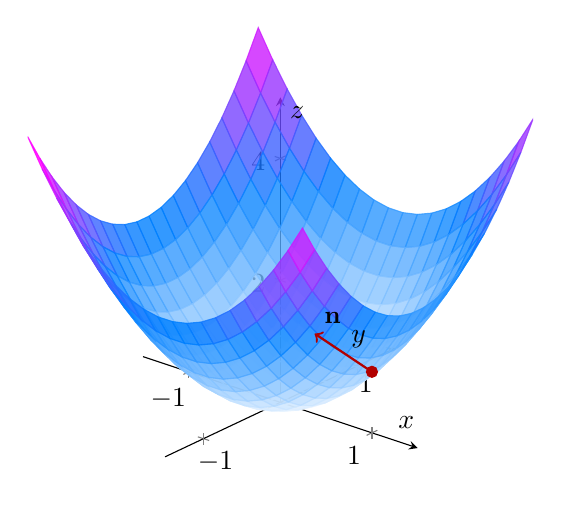
\begin{tikzpicture}
\begin{axis}[
    view={40}{25},
    xlabel={$x$}, ylabel={$y$}, zlabel={$z$},
    axis lines=center,
    tick style={thin},
    zmin=0, zmax=5,
    width=8cm, height=8cm,
]
    % Paraboloide z = x² + y²
    \addplot3[
        surf,
        shader=flat corner,
        samples=20,
        domain=-1.5:1.5,
        opacity=0.80,
        colormap/cool,
    ] {x^2 + y^2};

    % Punto sobre la superficie
    \addplot3[only marks, mark=*, mark size=2pt, red!70!black]
        coordinates {(1,0,1)};

    % Vector normal escalado ×0.7: (1,0,1)+(0.7·(−2,0,1)/√5)
    % ≈ (1−0.626, 0, 1+0.313) = (0.374, 0, 1.313)
    \draw[->, thick, red!70!black]
        (axis cs:1,0,1) -- (axis cs:0.374,0,1.313);
    \node[above right] at (axis cs:0.374,0,1.313)
        {\small $\mathbf{n}$};
\end{axis}
\end{tikzpicture}
\caption{Paraboloide $z=x^2+y^2$ con vector normal $\mathbf{n}$
         en el punto $(1,0,1)$}
\label{fig:paraboloide_normal}
\end{figure}

% ============================================================
% FIGURA C — Región tipo I: entre y=x² e y=x+2, x∈[−1,2]
% Uso previsto: integral doble, cambio de orden, área 2D
% TikZ puro (sin pgfplots) — sin overhead de axis 3D
% Opciones clave:
%   variable=\t + plot({\t},{expr}) → curva en TikZ puro
%   \path[fill] con plot--plot--cycle → relleno entre dos curvas
%   opacity=0.3 → región semitransparente sobre la grilla
%   \node separado del \draw → evita solapamiento de etiquetas
% Intersecciones: x²=x+2 → x=−1 (y=1) y x=2 (y=4)
% Posiciones de etiquetas:
%   $y=x^2$  → (2.2, 1.8) anchor=west  [derecha de la parábola, y=1.8]
%   $y=x+2$  → (0.5, 2.5) anchor=sw+yshift  [encima de la recta]
%   $(2,4)$  → anchor=west xshift=5pt  [derecha del punto]
% Tiempo de compilación: <1 s
% ============================================================
\begin{figure}[H]
\centering
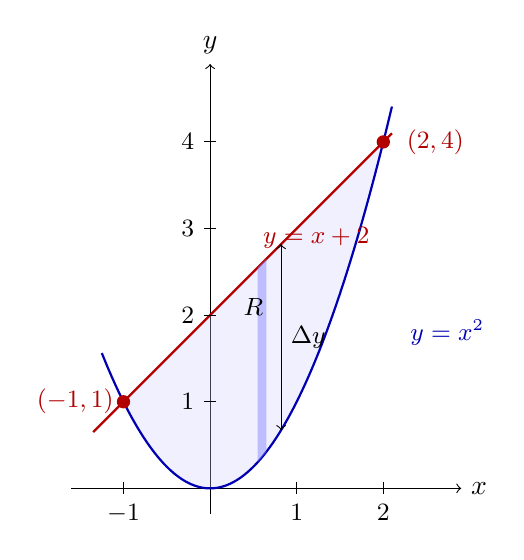
\begin{tikzpicture}[scale=1.1]
    % Ejes
    \draw[thin, ->] (-1.6,0) -- (2.9,0) node[right] {$x$};
    \draw[thin, ->] (0,-0.3) -- (0,4.9) node[above] {$y$};

    % Región sombreada: y=x+2 (arriba) sobre y=x² (abajo), x∈[−1,2]
    \path[fill=blue!20, opacity=0.30]
        plot[domain=-1:2, samples=40, smooth, variable=\t] ({\t},{\t+2})
        -- plot[domain=2:-1, samples=40, smooth, variable=\t] ({\t},{\t*\t})
        -- cycle;

    % Frontera inferior: parábola y = x²
    % Etiqueta en \node separado para evitar solapamiento con y=x+2 y (2,4)
    \draw[thick, blue!70!black, variable=\t,
          domain=-1.25:2.1, samples=50, smooth]
        plot ({\t},{\t*\t});
    \node[anchor=west, blue!70!black] at (2.2,1.8)
        {\small $y=x^2$};

    % Frontera superior: recta y = x + 2
    % Etiqueta sobre la recta en x=0.5, fuera de la región sombreada
    \draw[thick, red!70!black, variable=\t,
          domain=-1.35:2.1, samples=2]
        plot ({\t},{\t+2});
    \node[anchor=south west, red!70!black, yshift=5pt] at (0.5,2.5)
        {\small $y=x+2$};

    % Franja vertical representativa (x∈[0.55, 0.65])
    % Valores exactos: x=0.55 → y²=0.3025, y+2=2.55
    %                  x=0.65 → y²=0.4225, y+2=2.65
    \fill[blue!50, opacity=0.45]
        (0.55,0.3025)--(0.55,2.55)--(0.65,2.65)--(0.65,0.4225)--cycle;

    % Indicador de integración en y (flecha bilateral en x=0.82)
    \draw[<->, thin]
        (0.82,{0.82*0.82}) -- (0.82,{0.82+2})
        node[midway, right] {\small $\Delta y$};

    % Puntos de intersección
    \filldraw[red!70!black] (-1,1) circle (2pt)
        node[left] {\small $(-1,1)$};
    \filldraw[red!70!black] (2,4) circle (2pt)
        node[anchor=west, xshift=5pt] {\small $(2,4)$};

    % Marcas en eje x
    \foreach \xv in {-1,1,2}
        \draw[thin] (\xv,0.07)--(\xv,-0.07)
            node[below] {\small $\xv$};
    % Marcas en eje y
    \foreach \yv in {1,2,3,4}
        \draw[thin] (0.07,\yv)--(-0.07,\yv)
            node[left] {\small $\yv$};

    % Etiqueta de región
    \node at (0.5,2.1) {\small $R$};
\end{tikzpicture}
\caption{Región tipo I: área entre $y=x^2$ e $y=x+2$}
\label{fig:region_tipo_I}
\end{figure}

% ============================================================
% ESTÁNDARES GLOBALES DE FIGURAS — Libro Cálculo y AL
%
%   Superficies 3D : shader=flat o flat corner; samples≤20
%   Curvas 3D/2D  : samples=50, smooth
%   Etiquetas      : \small (nunca \footnotesize ni \normalsize)
%   Grosor:
%     thick  → curvas principales, flechas de campo, vectores
%     thin   → ejes, grillas, marcas de eje, flechas laterales
%   Paleta de colores:
%     blue!70!black → curvas / superficies principales
%     red!70!black  → vectores (tangente, normal, gradiente)
%     blue!20       → relleno de región (fill, opacity=0.3)
%     blue!50       → franja representativa (opacity=0.45)
%   Tiempo 3D: <15 s con shader=flat + samples=20 en LuaLaTeX
%   Entorno figure (obligatorio):
%     \begin{figure}[H]\centering ... \caption{}\label{fig:nombre}
%     \end{figure}  — [H] siempre; toda figura lleva caption y label
%   Etiquetas sin solapamiento (obligatorio):
%     Usar \node separado del \draw, nunca node al final de plot
%     Especificar anchor= explícito (west, south west, north, etc.)
%     Añadir xshift= / yshift= cuando haya riesgo de colisión
%     Verificar visualmente antes de cerrar el ítem
% ============================================================

% Requiere (ya en preámbulo principal):
%   \usepackage{pgf,tikz,pgfplots}  +  \pgfplotsset{compat=1.18}
%   \usetikzlibrary{arrows,...}     +  \usepackage{amsmath}
% Las tres figuras son plantillas de copia-pega independientes.
% ============================================================

% ============================================================
% FIGURA A — Hélice r(t)=(cos t, sin t, t/2) con tangente
% Uso previsto: curva en R³, función vectorial, trayectoria
% Opciones clave:
%   samples y=0  → curva 1D en 3D (no grilla de superficie)
%   deg(x)       → convierte rad a grados para sin/cos de pgfplots
%   axis cs:x,y,z → coordenadas del eje en \draw dentro de 3D
% Advertencia: ~4 s en LuaLaTeX (50 puntos en axis3d)
% ============================================================
\begin{figure}[H]
\centering
\begin{tikzpicture}
\begin{axis}[
    view={35}{20},
    xlabel={$x$}, ylabel={$y$}, zlabel={$z$},
    axis lines=center,
    tick style={thin},
    xtick={-1,0,1}, ytick={-1,0,1}, ztick={0,1,2,3},
    width=8cm, height=8cm,
]
    % Hélice parametrizada con variable interna x (rad)
    \addplot3[
        thick, blue!70!black,
        domain=0:6.2832,  % 0 a 2π en radianes
        samples=50,
        samples y=0,      % curva 1D, no superficie
    ] ({cos(deg(x))}, {sin(deg(x))}, {x/2});

    % Punto r(π/2) = (0, 1, π/4) ≈ (0, 1, 0.785)
    \addplot3[only marks, mark=*, mark size=2pt, red!70!black]
        coordinates {(0,1,0.785)};

    % Tangente r'(π/2)=(-1,0,1/2), escalada ×0.4
    % Extremo: (0-0.4, 1+0, 0.785+0.2) = (-0.4, 1, 0.985)
    \draw[->, thick, red!70!black]
        (axis cs:0,1,0.785) -- (axis cs:-0.4,1,0.985);
    \node[above left] at (axis cs:-0.4,1,0.985)
        {\small $\mathbf{r}'(\tfrac{\pi}{2})$};
\end{axis}
\end{tikzpicture}
\caption{Hélice $\mathbf{r}(t)=(\cos t,\sin t,\tfrac{t}{2})$,
         $t\in[0,2\pi]$, con vector tangente en $t=\tfrac{\pi}{2}$}
\label{fig:helice_tangente}
\end{figure}

% ============================================================
% FIGURA B — Paraboloide z=x²+y² con vector normal en (1,0,1)
% Uso previsto: plano tangente, flujo, normal a superficie
% Opciones clave:
%   surf, shader=flat corner → una tono por cara, sin interpolación
%   samples=20               → máximo recomendado (400 caras)
%   opacity=0.80             → deja ver los ejes subyacentes
%   colormap/cool            → paleta azul-cyan (reemplazar si gris)
% Normal: ∇(z−x²−y²)=(−2x,−2y,1) en (1,0,1)→(−2,0,1)/√5, ×0.7
% Advertencia: ~8 s en LuaLaTeX (superficie 3D con relleno)
% ============================================================
\begin{figure}[H]
\centering
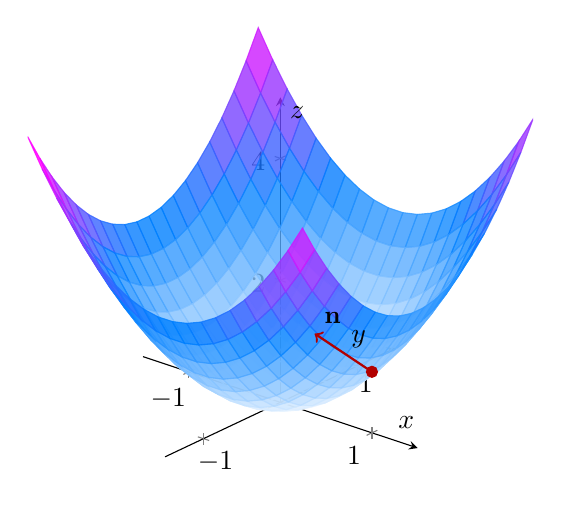
\begin{tikzpicture}
\begin{axis}[
    view={40}{25},
    xlabel={$x$}, ylabel={$y$}, zlabel={$z$},
    axis lines=center,
    tick style={thin},
    zmin=0, zmax=5,
    width=8cm, height=8cm,
]
    % Paraboloide z = x² + y²
    \addplot3[
        surf,
        shader=flat corner,
        samples=20,
        domain=-1.5:1.5,
        opacity=0.80,
        colormap/cool,
    ] {x^2 + y^2};

    % Punto sobre la superficie
    \addplot3[only marks, mark=*, mark size=2pt, red!70!black]
        coordinates {(1,0,1)};

    % Vector normal escalado ×0.7: (1,0,1)+(0.7·(−2,0,1)/√5)
    % ≈ (1−0.626, 0, 1+0.313) = (0.374, 0, 1.313)
    \draw[->, thick, red!70!black]
        (axis cs:1,0,1) -- (axis cs:0.374,0,1.313);
    \node[above right] at (axis cs:0.374,0,1.313)
        {\small $\mathbf{n}$};
\end{axis}
\end{tikzpicture}
\caption{Paraboloide $z=x^2+y^2$ con vector normal $\mathbf{n}$
         en el punto $(1,0,1)$}
\label{fig:paraboloide_normal}
\end{figure}

% ============================================================
% FIGURA C — Región tipo I: entre y=x² e y=x+2, x∈[−1,2]
% Uso previsto: integral doble, cambio de orden, área 2D
% TikZ puro (sin pgfplots) — sin overhead de axis 3D
% Opciones clave:
%   variable=\t + plot({\t},{expr}) → curva en TikZ puro
%   \path[fill] con plot--plot--cycle → relleno entre dos curvas
%   opacity=0.3 → región semitransparente sobre la grilla
%   \node separado del \draw → evita solapamiento de etiquetas
% Intersecciones: x²=x+2 → x=−1 (y=1) y x=2 (y=4)
% Posiciones de etiquetas:
%   $y=x^2$  → (2.2, 1.8) anchor=west  [derecha de la parábola, y=1.8]
%   $y=x+2$  → (0.5, 2.5) anchor=sw+yshift  [encima de la recta]
%   $(2,4)$  → anchor=west xshift=5pt  [derecha del punto]
% Tiempo de compilación: <1 s
% ============================================================
\begin{figure}[H]
\centering
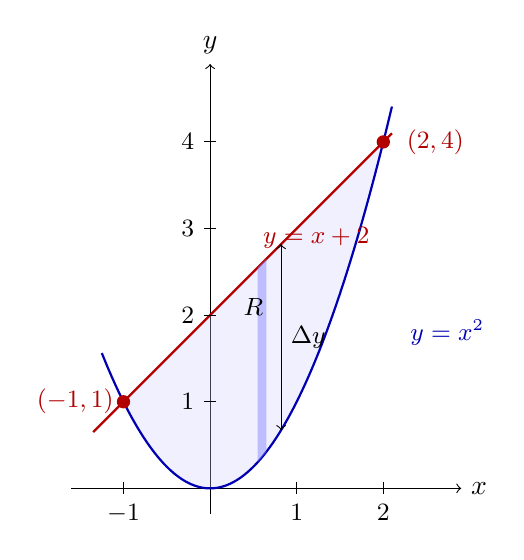
\begin{tikzpicture}[scale=1.1]
    % Ejes
    \draw[thin, ->] (-1.6,0) -- (2.9,0) node[right] {$x$};
    \draw[thin, ->] (0,-0.3) -- (0,4.9) node[above] {$y$};

    % Región sombreada: y=x+2 (arriba) sobre y=x² (abajo), x∈[−1,2]
    \path[fill=blue!20, opacity=0.30]
        plot[domain=-1:2, samples=40, smooth, variable=\t] ({\t},{\t+2})
        -- plot[domain=2:-1, samples=40, smooth, variable=\t] ({\t},{\t*\t})
        -- cycle;

    % Frontera inferior: parábola y = x²
    % Etiqueta en \node separado para evitar solapamiento con y=x+2 y (2,4)
    \draw[thick, blue!70!black, variable=\t,
          domain=-1.25:2.1, samples=50, smooth]
        plot ({\t},{\t*\t});
    \node[anchor=west, blue!70!black] at (2.2,1.8)
        {\small $y=x^2$};

    % Frontera superior: recta y = x + 2
    % Etiqueta sobre la recta en x=0.5, fuera de la región sombreada
    \draw[thick, red!70!black, variable=\t,
          domain=-1.35:2.1, samples=2]
        plot ({\t},{\t+2});
    \node[anchor=south west, red!70!black, yshift=5pt] at (0.5,2.5)
        {\small $y=x+2$};

    % Franja vertical representativa (x∈[0.55, 0.65])
    % Valores exactos: x=0.55 → y²=0.3025, y+2=2.55
    %                  x=0.65 → y²=0.4225, y+2=2.65
    \fill[blue!50, opacity=0.45]
        (0.55,0.3025)--(0.55,2.55)--(0.65,2.65)--(0.65,0.4225)--cycle;

    % Indicador de integración en y (flecha bilateral en x=0.82)
    \draw[<->, thin]
        (0.82,{0.82*0.82}) -- (0.82,{0.82+2})
        node[midway, right] {\small $\Delta y$};

    % Puntos de intersección
    \filldraw[red!70!black] (-1,1) circle (2pt)
        node[left] {\small $(-1,1)$};
    \filldraw[red!70!black] (2,4) circle (2pt)
        node[anchor=west, xshift=5pt] {\small $(2,4)$};

    % Marcas en eje x
    \foreach \xv in {-1,1,2}
        \draw[thin] (\xv,0.07)--(\xv,-0.07)
            node[below] {\small $\xv$};
    % Marcas en eje y
    \foreach \yv in {1,2,3,4}
        \draw[thin] (0.07,\yv)--(-0.07,\yv)
            node[left] {\small $\yv$};

    % Etiqueta de región
    \node at (0.5,2.1) {\small $R$};
\end{tikzpicture}
\caption{Región tipo I: área entre $y=x^2$ e $y=x+2$}
\label{fig:region_tipo_I}
\end{figure}

% ============================================================
% ESTÁNDARES GLOBALES DE FIGURAS — Libro Cálculo y AL
%
%   Superficies 3D : shader=flat o flat corner; samples≤20
%   Curvas 3D/2D  : samples=50, smooth
%   Etiquetas      : \small (nunca \footnotesize ni \normalsize)
%   Grosor:
%     thick  → curvas principales, flechas de campo, vectores
%     thin   → ejes, grillas, marcas de eje, flechas laterales
%   Paleta de colores:
%     blue!70!black → curvas / superficies principales
%     red!70!black  → vectores (tangente, normal, gradiente)
%     blue!20       → relleno de región (fill, opacity=0.3)
%     blue!50       → franja representativa (opacity=0.45)
%   Tiempo 3D: <15 s con shader=flat + samples=20 en LuaLaTeX
%   Entorno figure (obligatorio):
%     \begin{figure}[H]\centering ... \caption{}\label{fig:nombre}
%     \end{figure}  — [H] siempre; toda figura lleva caption y label
%   Etiquetas sin solapamiento (obligatorio):
%     Usar \node separado del \draw, nunca node al final de plot
%     Especificar anchor= explícito (west, south west, north, etc.)
%     Añadir xshift= / yshift= cuando haya riesgo de colisión
%     Verificar visualmente antes de cerrar el ítem
% ============================================================

% Requiere (ya en preámbulo principal):
%   \usepackage{pgf,tikz,pgfplots}  +  \pgfplotsset{compat=1.18}
%   \usetikzlibrary{arrows,...}     +  \usepackage{amsmath}
% Las tres figuras son plantillas de copia-pega independientes.
% ============================================================

% ============================================================
% FIGURA A — Hélice r(t)=(cos t, sin t, t/2) con tangente
% Uso previsto: curva en R³, función vectorial, trayectoria
% Opciones clave:
%   samples y=0  → curva 1D en 3D (no grilla de superficie)
%   deg(x)       → convierte rad a grados para sin/cos de pgfplots
%   axis cs:x,y,z → coordenadas del eje en \draw dentro de 3D
% Advertencia: ~4 s en LuaLaTeX (50 puntos en axis3d)
% ============================================================
\begin{figure}[H]
\centering
\begin{tikzpicture}
\begin{axis}[
    view={35}{20},
    xlabel={$x$}, ylabel={$y$}, zlabel={$z$},
    axis lines=center,
    tick style={thin},
    xtick={-1,0,1}, ytick={-1,0,1}, ztick={0,1,2,3},
    width=8cm, height=8cm,
]
    % Hélice parametrizada con variable interna x (rad)
    \addplot3[
        thick, blue!70!black,
        domain=0:6.2832,  % 0 a 2π en radianes
        samples=50,
        samples y=0,      % curva 1D, no superficie
    ] ({cos(deg(x))}, {sin(deg(x))}, {x/2});

    % Punto r(π/2) = (0, 1, π/4) ≈ (0, 1, 0.785)
    \addplot3[only marks, mark=*, mark size=2pt, red!70!black]
        coordinates {(0,1,0.785)};

    % Tangente r'(π/2)=(-1,0,1/2), escalada ×0.4
    % Extremo: (0-0.4, 1+0, 0.785+0.2) = (-0.4, 1, 0.985)
    \draw[->, thick, red!70!black]
        (axis cs:0,1,0.785) -- (axis cs:-0.4,1,0.985);
    \node[above left] at (axis cs:-0.4,1,0.985)
        {\small $\mathbf{r}'(\tfrac{\pi}{2})$};
\end{axis}
\end{tikzpicture}
\caption{Hélice $\mathbf{r}(t)=(\cos t,\sin t,\tfrac{t}{2})$,
         $t\in[0,2\pi]$, con vector tangente en $t=\tfrac{\pi}{2}$}
\label{fig:helice_tangente}
\end{figure}

% ============================================================
% FIGURA B — Paraboloide z=x²+y² con vector normal en (1,0,1)
% Uso previsto: plano tangente, flujo, normal a superficie
% Opciones clave:
%   surf, shader=flat corner → una tono por cara, sin interpolación
%   samples=20               → máximo recomendado (400 caras)
%   opacity=0.80             → deja ver los ejes subyacentes
%   colormap/cool            → paleta azul-cyan (reemplazar si gris)
% Normal: ∇(z−x²−y²)=(−2x,−2y,1) en (1,0,1)→(−2,0,1)/√5, ×0.7
% Advertencia: ~8 s en LuaLaTeX (superficie 3D con relleno)
% ============================================================
\begin{figure}[H]
\centering
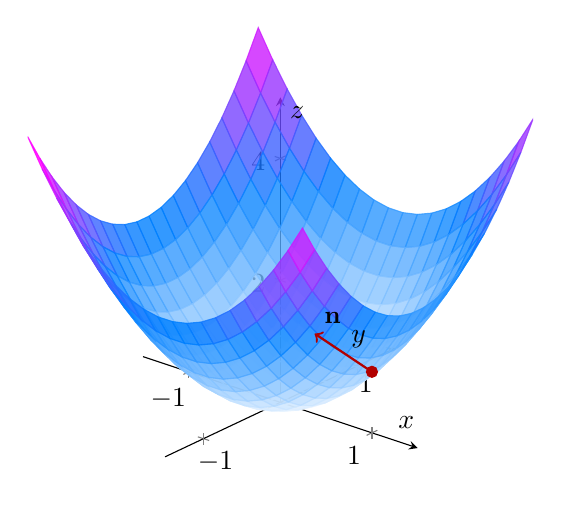
\begin{tikzpicture}
\begin{axis}[
    view={40}{25},
    xlabel={$x$}, ylabel={$y$}, zlabel={$z$},
    axis lines=center,
    tick style={thin},
    zmin=0, zmax=5,
    width=8cm, height=8cm,
]
    % Paraboloide z = x² + y²
    \addplot3[
        surf,
        shader=flat corner,
        samples=20,
        domain=-1.5:1.5,
        opacity=0.80,
        colormap/cool,
    ] {x^2 + y^2};

    % Punto sobre la superficie
    \addplot3[only marks, mark=*, mark size=2pt, red!70!black]
        coordinates {(1,0,1)};

    % Vector normal escalado ×0.7: (1,0,1)+(0.7·(−2,0,1)/√5)
    % ≈ (1−0.626, 0, 1+0.313) = (0.374, 0, 1.313)
    \draw[->, thick, red!70!black]
        (axis cs:1,0,1) -- (axis cs:0.374,0,1.313);
    \node[above right] at (axis cs:0.374,0,1.313)
        {\small $\mathbf{n}$};
\end{axis}
\end{tikzpicture}
\caption{Paraboloide $z=x^2+y^2$ con vector normal $\mathbf{n}$
         en el punto $(1,0,1)$}
\label{fig:paraboloide_normal}
\end{figure}

% ============================================================
% FIGURA C — Región tipo I: entre y=x² e y=x+2, x∈[−1,2]
% Uso previsto: integral doble, cambio de orden, área 2D
% TikZ puro (sin pgfplots) — sin overhead de axis 3D
% Opciones clave:
%   variable=\t + plot({\t},{expr}) → curva en TikZ puro
%   \path[fill] con plot--plot--cycle → relleno entre dos curvas
%   opacity=0.3 → región semitransparente sobre la grilla
%   \node separado del \draw → evita solapamiento de etiquetas
% Intersecciones: x²=x+2 → x=−1 (y=1) y x=2 (y=4)
% Posiciones de etiquetas:
%   $y=x^2$  → (2.2, 1.8) anchor=west  [derecha de la parábola, y=1.8]
%   $y=x+2$  → (0.5, 2.5) anchor=sw+yshift  [encima de la recta]
%   $(2,4)$  → anchor=west xshift=5pt  [derecha del punto]
% Tiempo de compilación: <1 s
% ============================================================
\begin{figure}[H]
\centering
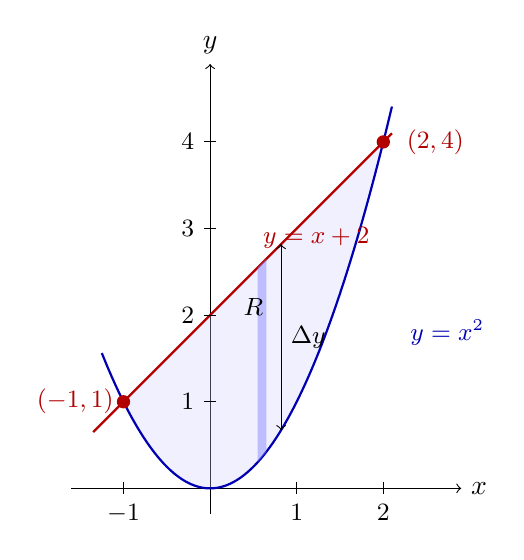
\begin{tikzpicture}[scale=1.1]
    % Ejes
    \draw[thin, ->] (-1.6,0) -- (2.9,0) node[right] {$x$};
    \draw[thin, ->] (0,-0.3) -- (0,4.9) node[above] {$y$};

    % Región sombreada: y=x+2 (arriba) sobre y=x² (abajo), x∈[−1,2]
    \path[fill=blue!20, opacity=0.30]
        plot[domain=-1:2, samples=40, smooth, variable=\t] ({\t},{\t+2})
        -- plot[domain=2:-1, samples=40, smooth, variable=\t] ({\t},{\t*\t})
        -- cycle;

    % Frontera inferior: parábola y = x²
    % Etiqueta en \node separado para evitar solapamiento con y=x+2 y (2,4)
    \draw[thick, blue!70!black, variable=\t,
          domain=-1.25:2.1, samples=50, smooth]
        plot ({\t},{\t*\t});
    \node[anchor=west, blue!70!black] at (2.2,1.8)
        {\small $y=x^2$};

    % Frontera superior: recta y = x + 2
    % Etiqueta sobre la recta en x=0.5, fuera de la región sombreada
    \draw[thick, red!70!black, variable=\t,
          domain=-1.35:2.1, samples=2]
        plot ({\t},{\t+2});
    \node[anchor=south west, red!70!black, yshift=5pt] at (0.5,2.5)
        {\small $y=x+2$};

    % Franja vertical representativa (x∈[0.55, 0.65])
    % Valores exactos: x=0.55 → y²=0.3025, y+2=2.55
    %                  x=0.65 → y²=0.4225, y+2=2.65
    \fill[blue!50, opacity=0.45]
        (0.55,0.3025)--(0.55,2.55)--(0.65,2.65)--(0.65,0.4225)--cycle;

    % Indicador de integración en y (flecha bilateral en x=0.82)
    \draw[<->, thin]
        (0.82,{0.82*0.82}) -- (0.82,{0.82+2})
        node[midway, right] {\small $\Delta y$};

    % Puntos de intersección
    \filldraw[red!70!black] (-1,1) circle (2pt)
        node[left] {\small $(-1,1)$};
    \filldraw[red!70!black] (2,4) circle (2pt)
        node[anchor=west, xshift=5pt] {\small $(2,4)$};

    % Marcas en eje x
    \foreach \xv in {-1,1,2}
        \draw[thin] (\xv,0.07)--(\xv,-0.07)
            node[below] {\small $\xv$};
    % Marcas en eje y
    \foreach \yv in {1,2,3,4}
        \draw[thin] (0.07,\yv)--(-0.07,\yv)
            node[left] {\small $\yv$};

    % Etiqueta de región
    \node at (0.5,2.1) {\small $R$};
\end{tikzpicture}
\caption{Región tipo I: área entre $y=x^2$ e $y=x+2$}
\label{fig:region_tipo_I}
\end{figure}

% ============================================================
% ESTÁNDARES GLOBALES DE FIGURAS — Libro Cálculo y AL
%
%   Superficies 3D : shader=flat o flat corner; samples≤20
%   Curvas 3D/2D  : samples=50, smooth
%   Etiquetas      : \small (nunca \footnotesize ni \normalsize)
%   Grosor:
%     thick  → curvas principales, flechas de campo, vectores
%     thin   → ejes, grillas, marcas de eje, flechas laterales
%   Paleta de colores:
%     blue!70!black → curvas / superficies principales
%     red!70!black  → vectores (tangente, normal, gradiente)
%     blue!20       → relleno de región (fill, opacity=0.3)
%     blue!50       → franja representativa (opacity=0.45)
%   Tiempo 3D: <15 s con shader=flat + samples=20 en LuaLaTeX
%   Entorno figure (obligatorio):
%     \begin{figure}[H]\centering ... \caption{}\label{fig:nombre}
%     \end{figure}  — [H] siempre; toda figura lleva caption y label
%   Etiquetas sin solapamiento (obligatorio):
%     Usar \node separado del \draw, nunca node al final de plot
%     Especificar anchor= explícito (west, south west, north, etc.)
%     Añadir xshift= / yshift= cuando haya riesgo de colisión
%     Verificar visualmente antes de cerrar el ítem
% ============================================================

% Requiere (ya en preámbulo principal):
%   \usepackage{pgf,tikz,pgfplots}  +  \pgfplotsset{compat=1.18}
%   \usetikzlibrary{arrows,...}     +  \usepackage{amsmath}
% Las tres figuras son plantillas de copia-pega independientes.
% ============================================================

% ============================================================
% FIGURA A — Hélice r(t)=(cos t, sin t, t/2) con tangente
% Uso previsto: curva en R³, función vectorial, trayectoria
% Opciones clave:
%   samples y=0  → curva 1D en 3D (no grilla de superficie)
%   deg(x)       → convierte rad a grados para sin/cos de pgfplots
%   axis cs:x,y,z → coordenadas del eje en \draw dentro de 3D
% Advertencia: ~4 s en LuaLaTeX (50 puntos en axis3d)
% ============================================================
\begin{figure}[H]
\centering
\begin{tikzpicture}
\begin{axis}[
    view={35}{20},
    xlabel={$x$}, ylabel={$y$}, zlabel={$z$},
    axis lines=center,
    tick style={thin},
    xtick={-1,0,1}, ytick={-1,0,1}, ztick={0,1,2,3},
    width=8cm, height=8cm,
]
    % Hélice parametrizada con variable interna x (rad)
    \addplot3[
        thick, blue!70!black,
        domain=0:6.2832,  % 0 a 2π en radianes
        samples=50,
        samples y=0,      % curva 1D, no superficie
    ] ({cos(deg(x))}, {sin(deg(x))}, {x/2});

    % Punto r(π/2) = (0, 1, π/4) ≈ (0, 1, 0.785)
    \addplot3[only marks, mark=*, mark size=2pt, red!70!black]
        coordinates {(0,1,0.785)};

    % Tangente r'(π/2)=(-1,0,1/2), escalada ×0.4
    % Extremo: (0-0.4, 1+0, 0.785+0.2) = (-0.4, 1, 0.985)
    \draw[->, thick, red!70!black]
        (axis cs:0,1,0.785) -- (axis cs:-0.4,1,0.985);
    \node[above left] at (axis cs:-0.4,1,0.985)
        {\small $\mathbf{r}'(\tfrac{\pi}{2})$};
\end{axis}
\end{tikzpicture}
\caption{Hélice $\mathbf{r}(t)=(\cos t,\sin t,\tfrac{t}{2})$,
         $t\in[0,2\pi]$, con vector tangente en $t=\tfrac{\pi}{2}$}
\label{fig:helice_tangente}
\end{figure}

% ============================================================
% FIGURA B — Paraboloide z=x²+y² con vector normal en (1,0,1)
% Uso previsto: plano tangente, flujo, normal a superficie
% Opciones clave:
%   surf, shader=flat corner → una tono por cara, sin interpolación
%   samples=20               → máximo recomendado (400 caras)
%   opacity=0.80             → deja ver los ejes subyacentes
%   colormap/cool            → paleta azul-cyan (reemplazar si gris)
% Normal: ∇(z−x²−y²)=(−2x,−2y,1) en (1,0,1)→(−2,0,1)/√5, ×0.7
% Advertencia: ~8 s en LuaLaTeX (superficie 3D con relleno)
% ============================================================
\begin{figure}[H]
\centering
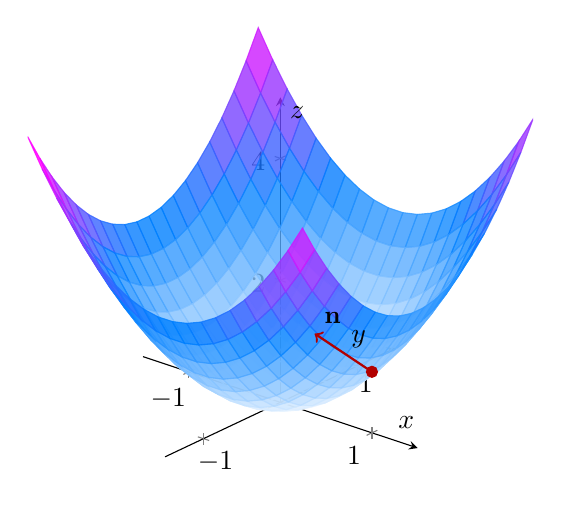
\begin{tikzpicture}
\begin{axis}[
    view={40}{25},
    xlabel={$x$}, ylabel={$y$}, zlabel={$z$},
    axis lines=center,
    tick style={thin},
    zmin=0, zmax=5,
    width=8cm, height=8cm,
]
    % Paraboloide z = x² + y²
    \addplot3[
        surf,
        shader=flat corner,
        samples=20,
        domain=-1.5:1.5,
        opacity=0.80,
        colormap/cool,
    ] {x^2 + y^2};

    % Punto sobre la superficie
    \addplot3[only marks, mark=*, mark size=2pt, red!70!black]
        coordinates {(1,0,1)};

    % Vector normal escalado ×0.7: (1,0,1)+(0.7·(−2,0,1)/√5)
    % ≈ (1−0.626, 0, 1+0.313) = (0.374, 0, 1.313)
    \draw[->, thick, red!70!black]
        (axis cs:1,0,1) -- (axis cs:0.374,0,1.313);
    \node[above right] at (axis cs:0.374,0,1.313)
        {\small $\mathbf{n}$};
\end{axis}
\end{tikzpicture}
\caption{Paraboloide $z=x^2+y^2$ con vector normal $\mathbf{n}$
         en el punto $(1,0,1)$}
\label{fig:paraboloide_normal}
\end{figure}

% ============================================================
% FIGURA C — Región tipo I: entre y=x² e y=x+2, x∈[−1,2]
% Uso previsto: integral doble, cambio de orden, área 2D
% TikZ puro (sin pgfplots) — sin overhead de axis 3D
% Opciones clave:
%   variable=\t + plot({\t},{expr}) → curva en TikZ puro
%   \path[fill] con plot--plot--cycle → relleno entre dos curvas
%   opacity=0.3 → región semitransparente sobre la grilla
%   \node separado del \draw → evita solapamiento de etiquetas
% Intersecciones: x²=x+2 → x=−1 (y=1) y x=2 (y=4)
% Posiciones de etiquetas:
%   $y=x^2$  → (2.2, 1.8) anchor=west  [derecha de la parábola, y=1.8]
%   $y=x+2$  → (0.5, 2.5) anchor=sw+yshift  [encima de la recta]
%   $(2,4)$  → anchor=west xshift=5pt  [derecha del punto]
% Tiempo de compilación: <1 s
% ============================================================
\begin{figure}[H]
\centering
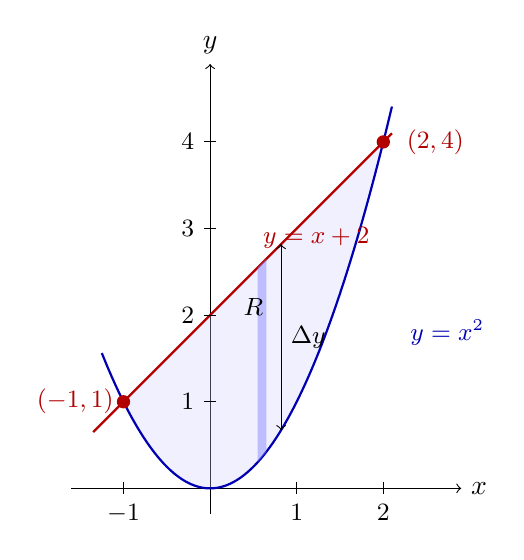
\begin{tikzpicture}[scale=1.1]
    % Ejes
    \draw[thin, ->] (-1.6,0) -- (2.9,0) node[right] {$x$};
    \draw[thin, ->] (0,-0.3) -- (0,4.9) node[above] {$y$};

    % Región sombreada: y=x+2 (arriba) sobre y=x² (abajo), x∈[−1,2]
    \path[fill=blue!20, opacity=0.30]
        plot[domain=-1:2, samples=40, smooth, variable=\t] ({\t},{\t+2})
        -- plot[domain=2:-1, samples=40, smooth, variable=\t] ({\t},{\t*\t})
        -- cycle;

    % Frontera inferior: parábola y = x²
    % Etiqueta en \node separado para evitar solapamiento con y=x+2 y (2,4)
    \draw[thick, blue!70!black, variable=\t,
          domain=-1.25:2.1, samples=50, smooth]
        plot ({\t},{\t*\t});
    \node[anchor=west, blue!70!black] at (2.2,1.8)
        {\small $y=x^2$};

    % Frontera superior: recta y = x + 2
    % Etiqueta sobre la recta en x=0.5, fuera de la región sombreada
    \draw[thick, red!70!black, variable=\t,
          domain=-1.35:2.1, samples=2]
        plot ({\t},{\t+2});
    \node[anchor=south west, red!70!black, yshift=5pt] at (0.5,2.5)
        {\small $y=x+2$};

    % Franja vertical representativa (x∈[0.55, 0.65])
    % Valores exactos: x=0.55 → y²=0.3025, y+2=2.55
    %                  x=0.65 → y²=0.4225, y+2=2.65
    \fill[blue!50, opacity=0.45]
        (0.55,0.3025)--(0.55,2.55)--(0.65,2.65)--(0.65,0.4225)--cycle;

    % Indicador de integración en y (flecha bilateral en x=0.82)
    \draw[<->, thin]
        (0.82,{0.82*0.82}) -- (0.82,{0.82+2})
        node[midway, right] {\small $\Delta y$};

    % Puntos de intersección
    \filldraw[red!70!black] (-1,1) circle (2pt)
        node[left] {\small $(-1,1)$};
    \filldraw[red!70!black] (2,4) circle (2pt)
        node[anchor=west, xshift=5pt] {\small $(2,4)$};

    % Marcas en eje x
    \foreach \xv in {-1,1,2}
        \draw[thin] (\xv,0.07)--(\xv,-0.07)
            node[below] {\small $\xv$};
    % Marcas en eje y
    \foreach \yv in {1,2,3,4}
        \draw[thin] (0.07,\yv)--(-0.07,\yv)
            node[left] {\small $\yv$};

    % Etiqueta de región
    \node at (0.5,2.1) {\small $R$};
\end{tikzpicture}
\caption{Región tipo I: área entre $y=x^2$ e $y=x+2$}
\label{fig:region_tipo_I}
\end{figure}

% ============================================================
% ESTÁNDARES GLOBALES DE FIGURAS — Libro Cálculo y AL
%
%   Superficies 3D : shader=flat o flat corner; samples≤20
%   Curvas 3D/2D  : samples=50, smooth
%   Etiquetas      : \small (nunca \footnotesize ni \normalsize)
%   Grosor:
%     thick  → curvas principales, flechas de campo, vectores
%     thin   → ejes, grillas, marcas de eje, flechas laterales
%   Paleta de colores:
%     blue!70!black → curvas / superficies principales
%     red!70!black  → vectores (tangente, normal, gradiente)
%     blue!20       → relleno de región (fill, opacity=0.3)
%     blue!50       → franja representativa (opacity=0.45)
%   Tiempo 3D: <15 s con shader=flat + samples=20 en LuaLaTeX
%   Entorno figure (obligatorio):
%     \begin{figure}[H]\centering ... \caption{}\label{fig:nombre}
%     \end{figure}  — [H] siempre; toda figura lleva caption y label
%   Etiquetas sin solapamiento (obligatorio):
%     Usar \node separado del \draw, nunca node al final de plot
%     Especificar anchor= explícito (west, south west, north, etc.)
%     Añadir xshift= / yshift= cuando haya riesgo de colisión
%     Verificar visualmente antes de cerrar el ítem
% ============================================================
